% Generated by experiments/exp2_thesis/make_assets.py -- do not edit by hand.
\begin{figure}[tbp]
  \centering
  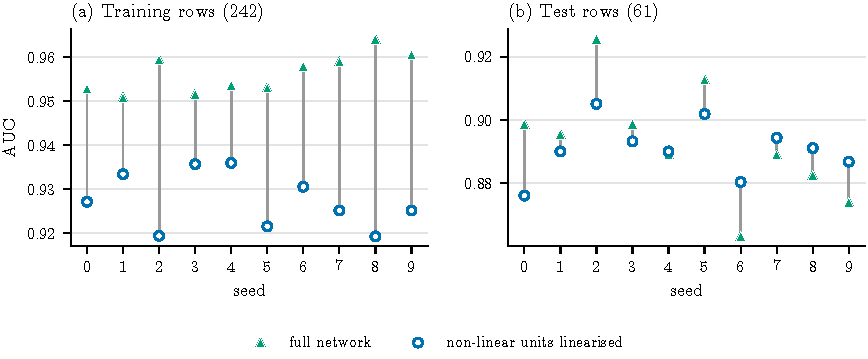
\includegraphics[width=\textwidth]{figures/exp2/exp2-heart-linearised}
  \caption{Heart-100: each network's AUC with and without its non-linear units (each replaced by its best straight line on the training rows). The non-linear units add 0.029 training AUC on average but 0.002 on test, and in 5 of the ten networks the linearised version does as well or better on test.}
  \label{fig:exp2-heart-linearised}
\end{figure}
